\documentclass{standalone}
\usepackage{tikz}
\usepackage{pxfonts}

\newcommand{\N}{\ensuremath{\mathbb{N}} }% set of natural numbers

\begin{document}
  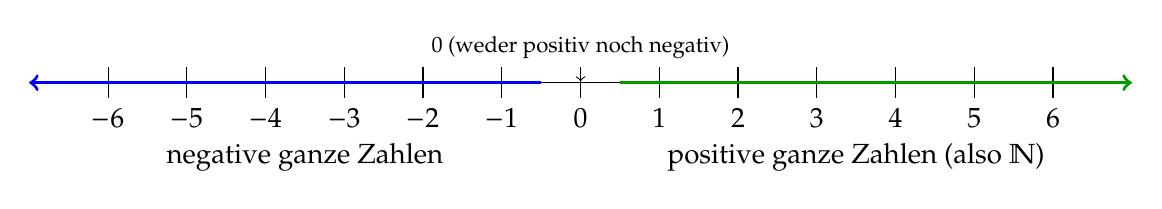
\begin{tikzpicture}%[scale = 8] 
\draw (-7,0) -- (7,0); 
\foreach \x in {-6,-5,-4,-3,-2,-1,0,1,2,3,4,5,6} \draw[shift={(\x,0)}] (0pt,.2) -- (0pt,-.2); 
\foreach \x in {-6,-5,-4,-3,-2,-1,0,1,2,3,4,5,6}
\draw[shift={(\x,-.2)}] node[below] {$\x$}; 
\draw[<-, very thick, blue] (-7,0) -- (-0.5,0); 
\draw[->, very thick, green!60!black] (0.5,0) -- (7,0); 
\draw[->] (0, 5 pt)node[above]{{\footnotesize 0 (weder positiv noch negativ)}} -- (0,1/2 pt);
\node at (-3.5, -.95) {negative ganze Zahlen};
\node at (3.5, -.95) {positive ganze Zahlen (also $\N$)};
\end{tikzpicture}
\end{document}
